\section{Maximum Mode Pins}
For using external coprocessors:
\begin{description}

    \item[$\overline{S2} , \overline{S1} and \overline{S0} $]
    \begin{itemize}
        \item Indicate the function of current bus-cycle
        \item Normally decoded by 8288 bus controllers
    \end{itemize}

    \item[$\overline{R1} / \overline{G1} and \overline{R0} / \overline{GT0} $]
    \begin{itemize}
        \item Request/grant pins
        \item Request Direct Memory Access
        \item Bi-Directional lines
        \item used to both request and grant a DMA operations
    \end{itemize}

    \item[$\overline{LOCK} $]
    \begin{itemize}
        \item Used to lock peripherals off the system
    \end{itemize}

    \item[$\overline{QS_1}$  and $\overline{QS0} $]
    \begin{itemize}
        \item Queue status bits
        \item Show status of the internal instructions queue
        \item Accessed by numeric coprocessor (8087)
    \end{itemize}

\end{description}

\begin{table}[h!]
\centering
\begin{tabular}{ |p{1cm}|p{1cm}|p{3cm}|  }
\hline
$ \overline{QS_1} $ & $ \overline{QS_0} $  & Function   \\
\hline
0 & 0 & Queue is idle \\
0 & 1 & First byte of opcode \\
1 & 0 & Queue is empty\\
1 & 1 & Subsequent byte of opcode \\
\hline
\end{tabular}

\caption{}
\label{table:4}
\end{table}

\section{Clock Generator (8284A)}
\begin{description}
  \item[Basic functions]
  \begin{itemize}
    \item Clock generation
    \item \textbf{RESET} synchronization
    \item READY synchronization
    \item TTL-level peripheral clock signal
  \end{itemize}
\end{description}
\newpage
\subsection{Pin diagram}
\begin{figure}[h!]
    \centering
    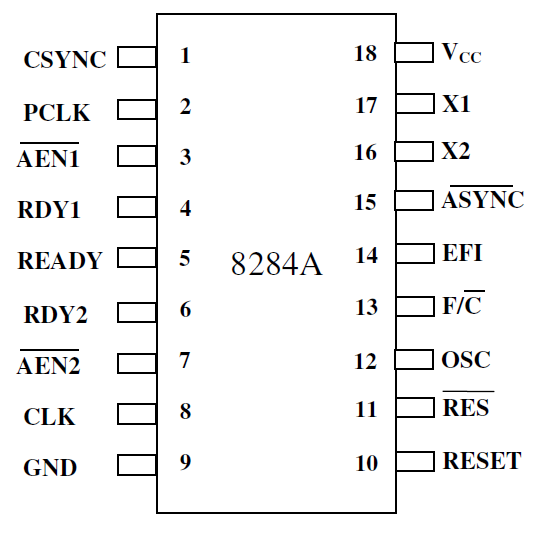
\includegraphics[width = 0.8\textwidth]{./figures/8284A.png}
    \caption{Pin Diagram for Intel 8284A}
    \label{fig:bl}
\end{figure}

\subsection{Pin Functions}
\begin{description}

  \item[AEN1 and AEN2]
  \begin{itemize}
    \item Qualify the bus ready signals, RDY1 and RDY2 respectively
    \item wait states are generated by the \textbf{READY} pin of $\mu P$, which is controlled
    by $\overline{AEN1}$ and $\overline{AEN2}$ pins
  \end{itemize}

  \item[RDY1 and RDY2]
  \begin{itemize}
    \item Bus ready inputs
    \item Cause wait states in conjunction with $\overline{AEN1}$ and $\overline{AEN2}$ pins
  \end{itemize}

  \item[$\overline{ASYNC}$]
  \begin{itemize}
    \item Ready synchronization
    \item Selects either one or two stages of synchronization for RDY1 and RDY2 inputs

  \end{itemize}

  \item[READY]
  \begin{itemize}
    \item An output pin that connects to the $\mu P's$ READY input
    \item Synchronized with RDY1 and RDY2 inputs
  \end{itemize}

  \item[X1 and X2]
  \begin{itemize}
    \item Crystal oscillator Pins
    \item Connect to an external crystal, which is used as the timing source for rhe clock generator and all its functions
  \end{itemize}

  \item[F/$\overline{C}$]
  \begin{itemize}
    \item Frequrncy/ crystal select input
    \item Chooses the clocking source
    \item If it is held high, and external clock is provided to the EFI pin.
    \item If it is held low, the internal crystal oscillator provides the timing signal.
  \end{itemize}

  \item[EFI]
  \begin{itemize}
    \item External frequency input
    \item Supplies timing whenever $F/\overline{C}$ pin is held high
  \end{itemize}

  \item[CLK]
  \begin{itemize}
    \item Clock output pin, which provides clock input tp $\mu P$ and other components
    \item Output signal and \textbf{one-third} of the crystal or EFI input frequency and has a duty cycle of 33\% (as required by 8086/8088)
  \end{itemize}

  \item[PCLK]
  \begin{itemize}
    \item Peripheral clock
    \item One sixth of the crystal of EFI input frequency, and has a 50\% duty cycle.
  \end{itemize}

  \item[OSC]
  \begin{itemize}
    \item Oscillator output
    \item At the same frequency as the crystal or EFI input
    \item Provides an EFI input to the other 8284A in a multiprocessor system.
  \end{itemize}

  \item[$\overline{RES}$]
  \begin{itemize}
    \item Reset input
    \item Often connected to an \textit{RC network} that provides power on resetting
  \end{itemize}

  \item[RESET]
  \begin{itemize}
    \item Reset output
    \item connected to the $\mu P'$s RESET input pin
  \end{itemize}

  \item[CSYNC]
  \begin{itemize}
    \item Clock synchronization
    \item Used whenever the EFI input provides synchronization in a multi-processor system
    \item If the \textit{internal oscillator} is used , this pin must be grounded.
  \end{itemize}


\end{description}
\section{Internal Block Diagram of 8284A Clock Generator}
\begin{figure}[h!]
    \centering
    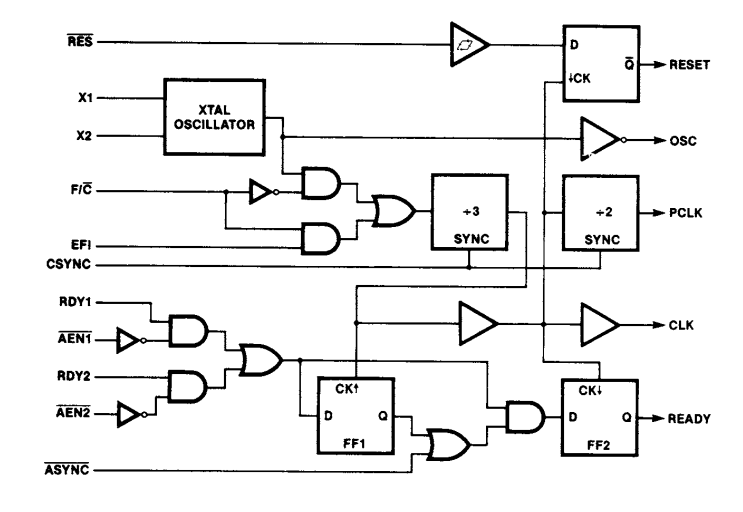
\includegraphics[width = 1.2\textwidth]{./figures/8284A_internal.png}
    \caption{Internal Block Diagram of 8284A Clock Generator}
    \label{fig:b2}
\end{figure}

\begin{itemize}
  \item If a crystal is attached to X1 and X2, the oscillator generates a square wave signal at the same frequenct as the crystal
  \item $CLK = \frac{frequency}{3}$ ; $PCLK = \frac{frequency}{6}$ ;
\end{itemize}
\newpage
\subsection{Operation of the RESET selection}
\begin{figure}[h!]
    \centering
    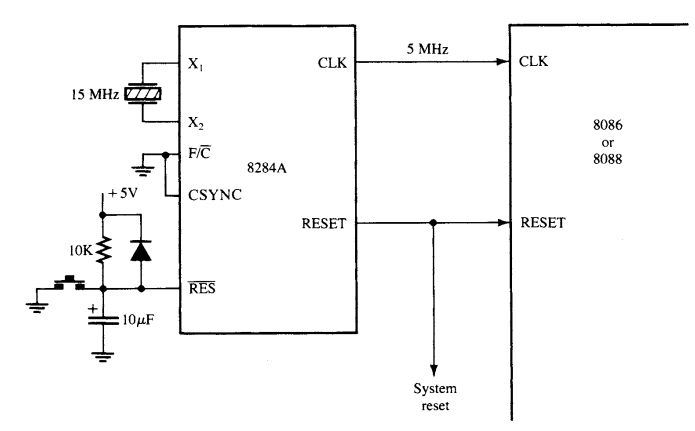
\includegraphics[width = 1.1\textwidth]{./figures/8284A_reset.png}
    \caption{The clock generator (8284A) and the 8086 and 8088 microprocessors illustrating
the connection for the clock and reset signals. A 15 MHz crystal provides the 5 MHz clock for the
microprocessor}
    \label{fig:b3}
\end{figure}

\begin{itemize}
  \item $\overline{RES}$ goes through a \textbf{Schmitt Trigger} and a D-type flip-flop, which ensures meeting timing requirements of the $\mu P's$ RESET input.
  \item The circuit applies RESET to the $\mu P$ at tghe negative edge ($1 \longrightarrow 0$),and the $\mu P$ samples the RESET signal at the positive edge ($0 \longrightarrow 1$)
  \item When power is first applied to the system, the RC circuit provides a \textbf{logic 0} to the $\overline{RES}$
  \item After a short time, $\overline{RES}$ becomes \textbf{logic 1}, as the capacitor charges to the $+5V$ through the resistor
  \item The push allows the $\mu P$ to be reset by an operator
  \item Correct RESET timing requires the RESET input to become a \textbf{logic 1} no later then 4 clock cycles after the power is applied, and held high for atleast $50 \mu s$
  \item RESET goes high in 4 clock cycles: by FF
  \item RESET stays high for $50 \mu s$: by RC time constant.
\end{itemize}
